\chapter{Estado del Arte}\label{chapter:state-of-the-art}

El proceso de construir modelos de \textit{machine learning} de gran calidad es complejo, iterativo y consume gran cantidad de tiempo, ya que este proceso está conformado por varios pasos. Los científicos de datos necesitan recolectar los datos y limpiarlos, seleccionar el algoritmo que mejor se ajuste a la tarea entre una cantidad enorme de algoritmos, ya sean técnicas de regresión, clasificación, de agrupamiento etc; además de afinar numerosos parámetros del algoritmo seleccionado y posteriormente aplicar numerosas métricas con el objetivo de juzgar el proceso de construcción del modelo. Por lo que la decisión del científico de dato en cada paso afecta directamente la construcción de un modelo de calidad, entonces diferentes combinaciones de estos producen diferentes valores en las métricas que se evaluan. \\

Explorar todas las combinaciones posibles para resolver un problema muchas veces es no viable, ya que puede ser exponencial la cantidad de configuraciones en las cuales se puede evaluar nuestro problema, cada combinación conlleva al consumo de recursos computacionales y de tiempo. \\

La automatización de este proceso es llamado AutoML o Auto Machine Learning. Es importante saber que AutoML no es una tendencia nueva. En los años 1990s, soluciones comerciales ofrecían automatizar HPO para algoritmos de clasificación seleccionados vía \textit{grid search} \parencite{17}. Adaptaciones al \textit{grid search} para probar posibles configuraciones en un enfoque \textit{greedy} están disponibles desde 1995 \parencite{18}. Temprano en los 2000s las primeras estrategias eficientes para HPO fueron propuestas. Para configuraciones limitadas, por ejemplo afinar $C$ y $\gamma$ de un \textit{support vector machine} (SVM) \parencite{19} \parencite{20}, fue probado que las estrategias de búsqueda guiadas tienen mejor resultado que \textit {grid search} en menor tiempo. También en el 2004, el primer enfoque para automatizar la selección de características fue publicado \parencite{21}. Selección completa del modelo \parencite{22} fue el primer intento de construir automáticamente un pipeline de ML completo seleccionando un algoritmo de preprocesamiento, de selección de características y de clasificación simultáneamente, mientras se afinaban los hiperparámetros de cada uno de estos algoritmos. Evaluando este enfoque en varios conjuntos de datos se demostró el potencial de este método \parencite{23}. Iniciando el 2011 muchos métodos diferentes aplicando optimización Bayesiana para la afinación de hiperparámetros \parencite{24} \parencite{8} y selección de modelos fueron propuestos \parencite{13}. En el 2015, el primer método de ingeniería de características automático sin conocimiento del dominio fue propuesto \parencite{26}. Es posible construir pipelines de forma variable desde el 2016 \parencite{27}. En el 2017 y 2018 el tema de AutoML recibió mucha atención en los medios con la realización de soluciones comerciales de AutoML \parencite{28} \parencite{29} \parencite{30} \parencite{31}. Simultáneamente las investigaciones en el área de AutoML ganaron mucha atracción conllevando a mejoras de rendimiento significativas. Métodos recientes son capaces de reducir el tiempo de corrida de procedimientos AutoML desde varias horas a algunos minutos \parencite{32}.

\section{AutoML como problema CASH}

El AutoML como problema CASH o \textit{Combined Algorithm Selection and Hyperparameter Optimization} fue introducido por Auto-Weka el cual define dos procesos importantes en la etapa de AutoML, la selección del modelo(\textit{Model Selection}, ML) y la optimización de hiperparámetros (\textit{Hyperparameter Optimization}, HPO).

\subsection{Model Selection:}
Dado un conjunto de algoritmos de \textit{machine learning} $\mathcal{A}$ y una limitada cantidad de datos de entrenamiento $\mathcal{D} = \{(x_1, y_1), ..., (x_n, y_n)\}$ el objetivo de la selección del modelo es determinar el algoritmo $A^* \in \mathcal{A}$ con un desempeño general óptimo. El desempeño general es estimado dividiendo $\mathcal{D}$ en conjuntos disjuntos de entrenamiento y validación $\mathcal{D}^{i}_{train}$ y $\mathcal{D}^{i}_{valid}$, funciones $f_i$ que aprenden al aplicar $A^*$ a $\mathcal{D}^{i}_{train}$ y evaluar el desempeño predictivo de estas funciones en $\mathcal{D}^{i}_{valid}$. Esto permite escribir el problema de selección del modelo de la siguiente forma:

$$A^* \in \argmin_{A \in \mathcal{A}} \frac{1}{k} \sum^{k}_{i = 1} \mathcal{L}(A, \mathcal{D}^{i}_{train}, \mathcal{D}^{i}_{valid}) $$
Donde $\mathcal{L}(A, \mathcal{D}^{i}_{train}, \mathcal{D}^{i}_{valid})$ es la pérdida obtenida por $A$ cuando fue entrenada con $\mathcal{D}^{i}_{train}$ y evaluada en $\mathcal{D}^{i}_{valid}$.

\subsection{Hyperparameter Optimization:}
El problema de optimización de hiperparámetros $\lambda \in \Lambda$ de un algoritmo de \textit{machine learning} $A$ es conceptualmente similar al problema de selección del modelo. Algunas diferencias claves son que los hiperparámetros a menudo son valores contínuos, que el espacio de hiperparámetros es de grandes dimensiones y que se puede explotar la correlación entre distintas configuraciones de parámetros. Dados $n$ hiperparámetros $\lambda_1, ..., \lambda_{n}$ con dominios $\Lambda_1, ..., \Lambda_n$ el espacio de hiperparámetros $\lambda$ es un subconjunto del producto cruzado de estos dominios $\Lambda \subset \Lambda_1 \times ... \times \Lambda_n$. Este subconjunto es a menudo estricto, tal que algunas configuraciones de hiperparámetros hacen inactivos a otros hiperparámetros. Más formalmente, se dice que un hiperparámetro $\lambda_i$ es condicional en otro hiperparámetro $\lambda_j$ si $\lambda_i$ está activo si el hiperparámetro $\lambda_j$ toma valores en un conjunto dado $V_i(j) \subset \Lambda_j$. Dando lugar a un espacio en forma de árbol o algunas veces en forma de grafo dirigido acíclico(DAG). Dado un espacio $\Lambda_{A}$ el problema de optimización de hiperparámetros puede ser escrito como:
$$\lambda^* \in \argmin_{\lambda \in \Lambda} \frac{1}{k} \sum^{k}_{i = 1} \mathcal{L}(A_{\lambda}, \mathcal{D}^{i}_{train}, \mathcal{D}^{i}_{valid}) $$.

\section{Componentes del proceso de AutoML}
En el proceso de AutoML destacan tres tareas importantes, la primera es el espacio de búsqueda el cual representa el conjunto de todas las posibles combinaciones que pueden resolver nuestro problema, la segunda es la estrategia de búsqueda que tiene como objetivo encontrar soluciones en el espacio de búsqueda de forma óptima y la tercera es la métrica de rendimiento que se utiliza para comparar que tan buena puede ser una solución con respecto a otra.

\subsection{Espacio de búsqueda}
La búsqueda de espacio define un paradigma estructural que los métodos de optimización de arquitecturas pueden explorar, por lo que diseñar un buen espacio de búsqueda es un problema retador de vital importancia. En general de un buen espacio de búsqueda se espera que excluya el sesgo humano y que sea lo suficientemente flexible para cubrir una gran variedad de arquitecturas de modelos.

Un espacio de búsqueda relativamente sencillo es el espacio de redes neuronales con estrucutra de cadenas(\textit{chain-structured neural network}). Una arquitectura de red neuronal con estructura de cadena puede ser escrita como una secuencia de capas, donde la $i$-th capa $L_i$ recibe en su entrada la salida de la capa $L_{i-1}$, y su salida sirve como entrada de la capa $L_{i + 1}$. Entonces el espacio de búsqueda está parametrizado por:

\begin{itemize}
\item El máximo número de capas.
\item El tipo de operación que cada capa ejecuta.
\item Los hiperparámetros asociados con la operación (p.e. número de filtros, tamaño del kernel). Los parámetros son condicionados por lo que el espacio de búsqueda es condicional.
\end{itemize}

Trabajos recientes en NAS (\parencite{56} \parencite{65} \parencite{66} \parencite{67} \parencite{68}) incorporan elementos de diseño moderno conocidos como arquitecturas \textit{hand-crafted}, como conexiones de satlo que permiten construir redes de múltiples ramas. En este caso la entrada de la capa $i$ puede ser descrita como una función que combina la salida de capas anteriores. El empleo de tal función da como resultado más grados de libertad.\\

Consecuentemente, este espacio de búsqueda basado en celdas es también empleado exitosamente por muchos trabajos recientes \parencite{68} \parencite{37} \parencite{62} \parencite{67} \parencite{69}. Sin embargo, surge una nueva elección de diseño cuando se utiliza un espacio de búsqueda basado en celdas, cómo elegir la macroarquitectura: ¿cuántas celdas se utilizarán y cómo se conectarán para construir el modelo real. Por ejemplo, \parencite{56} construyen un modelo secuencial a partir de celdas, en el que cada celda recibe como entrada las salidas de las dos celdas anteriores, mientras que \parencite{69} emplean la estructura de alto nivel de arquitecturas conocidas manualmente diseñadas, como DenseNet \parencite{70}, y usan sus celdas dentro de estos modelos. Un paso en la dirección de optimizar las macroarquitecturas es el espacio de búsqueda jerárquico introducido por \parencite{38}, que consta de varios niveles de motivos. El primer nivel consta del conjunto de operaciones primitivas, el segundo nivel de diferentes motivos que conectan operaciones primitivas a través de un DAG, el tercer nivel de motivos que codifican cómo conectar motivos de segundo nivel, y así sucesivamente. El espacio de búsqueda basado en celdas puede verse como un caso especial de este espacio de búsqueda jerárquico donde el número de niveles es tres, los motivos del segundo nivel corresponden a las celdas y el tercer nivel es la macroarquitectura codificada. \\
La elección del espacio de búsqueda determina en gran medida la dificultad del problema de optimización: incluso para el caso del espacio de búsqueda basado en una sola celda con macroarquitectura fija, el problema de optimización sigue siendo discontinuo y con dimensiones relativamente altas.


\subsection{Estrategia de búsqueda}

Las técnicas de aprendizaje profundo constituyen un subconjunto de metodologías de \textit{machine learning} que son basadas en redes neuronales artificiales (ANN) las cuales principalmente fueron inspiradas en la arquitectura del cerebro humano \parencite{34}. Se describe como profundo porque tiene más de una capa de transformaciones de características no lineales. Búsqueda de arquitecturas neuronales (NAS) es un paso fundamental en la automatización de los procesos de \textit{machine learning} y ha sido exitosamente usado para el diseño de arquitecturas de modelos para imágenes y tareas del lenguaje \parencite{35} \parencite{36} \parencite{37} \parencite{38} \parencite{39}. Las técnicas NAS recaen en 5 principales categorías que incluyen, \textit{random search}, aprendizaje por reforzamiento, métodos basados en gradiente, métodos evolutivos y métodos de optimización Bayesiana.

\begin{figure}[H]
    \center 
    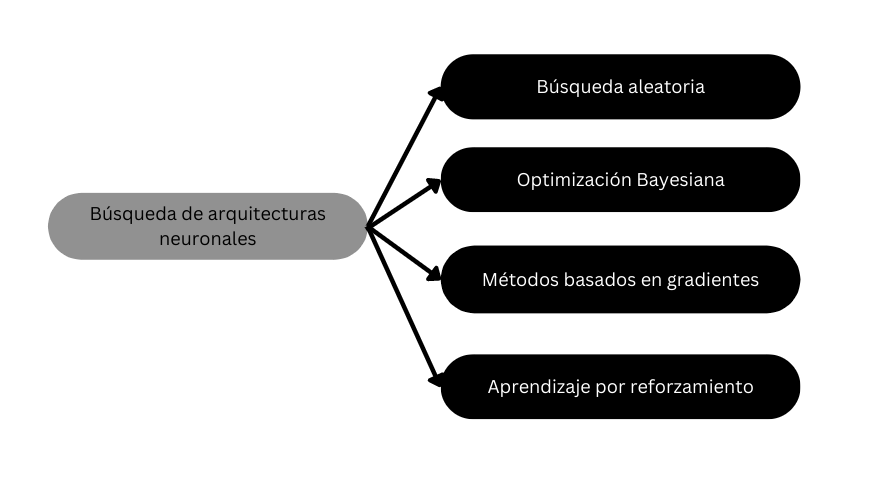
\includegraphics[scale=0.4]{images/NAS.png}
    \caption{Técnicas de arquitecturas de redes neuronales}
\end{figure}

\textit{Random search} es uno de los enfoques más ingenuos y simples para la búsqueda de arquitectura de red. Por ejemplo, \parencite{40} han presentado un enfoque para encontrar una buena arquitectura de red mediante la búsqueda aleatoria combinada con un conjunto bien entrenado de pesos compartidos. \parencite{41} propusieron nuevas líneas de base de búsqueda de arquitectura de red que se basan en la búsqueda aleatoria con parada anticipada para la optimización de hiperparámetros. Los resultados muestran que la búsqueda aleatoria junto con la parada anticipada logra resultados de búsqueda de arquitectura de red en el estado del arte en dos marcadores NAS estándar..

\textit{Reinforcement Learning} \parencite{42} es otro enfoque que se ha utilizado para encontrar la mejor arquitectura de red. \parencite{43} utilizaron una red neuronal recurrente (LSTM) con refuerzo para componer la arquitectura de la red neuronal. Más específicamente, la red neuronal recurrente se entrena a través de un algoritmo de búsqueda basado en gradiente llamado REINFORCE \parencite{44} para maximizar la precisión esperada de la arquitectura de la red neuronal generada. \parencite{45} introdujo un algoritmo de \textit{meta-modeling} llamado MetaQNN basado en el aprendizaje por refuerzo para generar automáticamente la arquitectura de la red neuronal convolucional para una nueva tarea. Las capas de la red neuronal convolucional son elegidas secuencialmente por un agente de aprendizaje que está entrenado usando \textit{Q-learning} con una técnica de exploración $\mathcal{E}$-\textit{greedy}. Simplemente, el agente explora un espacio de búsqueda finito de un conjunto de arquitecturas e iterativamente descubre diseños de arquitectura con un rendimiento mejorado en la nueva tarea a aprender.

\textit{Gradient-based optimization} es otra forma común para búsquedas de arquitecturas de redes neuronales. \parencite{46} propuso un enfoque basado en la relajación contínua de la arquitectura neuronal permitiendo usar descenso del gradiente para la búsqueda de la arquitectura. Los experimentos mostraron que este enfoque sobresale en encontrar arquitecturas convolucionales de alto rendimiento para la clasificación de imágenes en CIFAR-10, y en los conjuntos de datos de \textit{ImageNet}. \parencite{47} propuso un enfoque de optimización del descenso del gradiente para aprender la arquitectura de la red y parámetros simultáneamente. \parencite{48} usaron un enfoque basado en el gradiente para aprender arquitectura de redes. Los resultados experimentales en dos arquitecturas de redes diferentes: \textit{ResNet} y \textit{ResNeXt} mostraron que este enfoque recae en mejor precisión una reducción significativa en el número de parámetros. 

\textit{Bayesian optimization} basado en procesos \textit{Gaussian} ha sido usado por \parencite{49} y \parencite{50} para abordar el problema de búsqueda de arquitectura de redes neuronales. En adición, muchos trabajos se enfocaron en usar modelos basados en árboles como \textit{random forests} y \textit{tree Parzen estimators} \parencite{51} para efectivamente optimizar la arquitectura de red al igual que sus hiperparámetros \parencite{52} \parencite{53} \parencite{54}. La optimización Bayesiana  puede superar a algoritmos evolutivos en algunos problemas \parencite{55}

\subsection{Estrategia de rendimiento}
El objetivo de NAS es típicamente encontrar arquitecturas que puedan obtener alto rendimiento en la predicción de datos no vistos. La opción simple es ejecutar un entrenamiento estándar y la validación de la arquitectura en los datos, pero esto desafortunadamente es costoso computacionalmente y limita el número de arquitecturas que pueden ser exploradas. Investigaciones más recientes se enfocan en el desarrollo de métodos que reducen el costo de estas estimaciones de rendimiento. \\

El rendimiento puede ser estimado basado en \textit{lower fidelities} del actual rendimiento luego de un entrenamiento completo(también llamado \textit{proxy metrics}). Estas \textit{lower fidelities} incluyen menor tiempo de entrenamiento (\parencite{56} \parencite{57}), entrenar un subconjunto de los datos \parencite{58}, en imágenes de baja resolución \parencite{59}, o con menos filtros por capa y menos celdas. Mientras estas aproximaciones \textit{low-fidelity} reducen el costo computacional, también introducen un sesgo en la estimación, ya que normalmente se subestima el rendimiento. Esto puede que no sea problemático siempre que la estrategia de búsqueda solo se base en clasificar diferentes arquitecturas y la clasificación relativa permanezca estable. Sin embargo, resultados recientes indican que esta clasificación relativa puede cambiar drásticamente cuando la diferencia entre las aproximaciones baratas y la evaluación “completa” es demasiado grande \parencite{57}, lo que aboga por un aumento gradual de las fidelidades \parencite{60} \parencite{61}.\\

Otra estrategia aplicada con éxito a las redes neuronales convolucionales (Convolutional Neural Networks, CNN) es compartir pesos entre diferentes modelos, lo que se conoce como compartición de parámetros o compartición de pesos \parencite{62}. Para NAS diferenciables con un gran modelo one-shot, la compartición de parámetros se logra naturalmente ya que las arquitecturas y los pesos se entrenan conjuntamente. Sin embargo, entrenar el modelo one-shot puede ser difícil ya que contiene todas las operaciones posibles. Para acelerar aún más el proceso de entrenamiento, \textit{single-path one-shot} fue propuesto \parencite{63} en el que solo se activa una operación entre un par de entrada y salida durante cada paso. Para NAS sin un modelo \textit{one-shot}, compartir pesos entre diferentes arquitecturas es más difícil pero no del todo imposible. Por ejemplo, dado que se sabe que algunos filtros convolucionales son extractores de características comunes, heredar pesos de arquitecturas anteriores es factible y razonable en las CNN \parencite{64}. 

\section{Sistemas AutoML}
En esta sección se describen algunos sistemas de AutoML, los cuales fueron elegidos según su popularidad, son \textit{frameworks AutoML} capaces de construir \textit{pipelines} completos de \textit{machine learning}:

\subsection{Auto-Weka} 
Auto-Weka \parencite{13} considera una amplia gama de técnicas de selección de características (que combinan 3 métodos de búsqueda y 8 de evaluación) y todos los enfoques de clasificación implementados en la librería WEKA, que abarcan 2 métodos de conjunto, 10 metamétodos, 27 clasificadores básicos y configuraciones de hiperparámetros para cada clasificador.   

El software de aprendizaje automático WEKA pone técnicas de \textit{machine learning} de última generación a disposición incluso de los usuarios más novatos. Sin embargo, estos usuarios normalmente no saben cómo elegir entre las docenas de procedimientos de \textit{machine learning} implementados en WEKA y la configuración de hiperparámetros de cada procedimiento para lograr un buen rendimiento. Auto-WEKA aborda este problema al tratar todo WEKA como un único marco de aprendizaje automático altamente paramétrico, y al usar la optimización bayesiana para encontrar una instancia sólida para un conjunto de datos determinado.

Desde el lanzamiento inicial de un prototipo de investigación utilizable en 2013 \parencite{13}, se han realizado mejoras sustanciales en el paquete Auto-WEKA. En un nivel prosaico, se han corregido errores, mejorado las pruebas y la documentación, y actualizado el software para que funcione con las últimas versiones de WEKA y Java. También se han agregado cuatro características principales.

Primero, ahora se admiten algoritmos de regresión, expandiendo Auto-WEKA más allá de su enfoque anterior en la clasificación. En segundo lugar, ahora se admite la optimización de todas las métricas de rendimiento que admite WEKA. En tercer lugar, ahora se admite ejecuciones paralelas de forma nativa(en una sola máquina) para encontrar buenas configuraciones más rápido y guardar las $N$ mejores configuraciones de cada ejecución en lugar de solo la mejor. Cuarto, Auto-WEKA 2.0 ahora está completamente integrado con WEKA. Esto es importante, porque el quid de Auto-WEKA radica en su simplicidad: proporciona una interfaz de botón que no requiere conocimiento sobre los algoritmos de aprendizaje disponibles o sus hiperparámetros, y le pide al usuario que proporcione, además del conjunto de datos que se procesará, solo un límite de memoria (1 GB de forma predeterminada) y el presupuesto de tiempo general disponible para todo el proceso de aprendizaje. El presupuesto general se establece en 15 minutos de forma predeterminada para acomodar a los usuarios impacientes; las ejecuciones más largas permiten que el optimizador bayesiano busque en el espacio más a fondo.

La facilidad de uso del prototipo de investigación anterior se vio obstaculizada por el hecho de que los usuarios tenían que descargar Auto-WEKA manualmente y ejecutarlo por separado de WEKA. Por el contrario, Auto-WEKA 2.0 está disponible a través del administrador de paquetes de WEKA. Los usuarios no necesitan instalar el software por separado; todo está incluido en el paquete y se instala automáticamente a pedido. Después de la instalación, Auto-WEKA 2.0 se puede utilizar de dos maneras diferentes:
\begin{itemize}
    \item Como metaclasificador: Auto-WEKA se puede ejecutar como cualquier otro algoritmo de aprendizaje automático en WEKA: a través de la GUI, la interfaz de línea de comandos o la API pública. La figura 2 muestra cómo ejecutarlo desde la línea de comandos.
    \item A través de la pestaña Auto-WEKA: Esto proporciona una interfaz personalizada que oculta parte de la complejidad. La figura 3 muestra el resultado de una ejecución de ejemplo.
\end{itemize}

El código fuente de Auto-WEKA está alojado en GitHub (https://github.com/automl/autoweka) y está disponible bajo la licencia GPL (versión 3). Los lanzamientos se publican en el repositorio de paquetes WEKA y están disponibles a través del administrador de paquetes WEKA y del sitio web del proyecto Auto-WEKA (http://automl.org/autoweka).

\subsection{TPOT} 
TPOT \parencite{27} es un sistema AutoML de código abierto basado en programación genética que optimiza una serie de preprocesadores de características y modelos de \textit{machine learing} con el objetivo de maximizar la precisión de clasificación en una tarea de clasificación supervisada.

\subsection{Hyperopt-Sklearn} 
Hyperopt-sklearn \parencite{74} es un proyecto de software que proporciona una configuración automática de algoritmos de la biblioteca de \textit{machine learning} de \textit{Scikit-learn}. Siguiendo a \textit{Auto-Weka}, se considera que la elección del clasificador e incluso la elección del módulo de preprocesamiento se pueden tomar en conjunto para representar un único gran problema de optimización de hiperparámetros. Hyperopt se usa para definir un espacio de búsqueda que abarca muchos componentes estándar (por ejemplo, SVM, RF, KNN, PCA, TFIDF) y patrones comunes para componerlos juntos. Mejoró las puntuaciones más conocidas para el espacio modelo tanto para \textit{MNIST} como para \textit{Convex Shapes}.

La biblioteca \textit{Hyperopt} ofrece algoritmos de optimización para espacios de búsqueda que surgen en la configuración de algoritmos. Estos espacios se caracterizan por una variedad de tipos de variables (continuas, ordinales, categóricas), diferentes perfiles de sensibilidad (por ejemplo, escalado uniforme versus logarítmico) y estructura condicional (cuando se puede elegir entre dos clasificadores, los parámetros de un clasificador son irrelevantes cuando se elige el otro clasificador).

\subsection{Auto-Sklearn} 
Auto-Sklearn \parencite{6} es un sistema AutoML basado en \textit{scikit-learn} (que utiliza 15 clasificadores, 14 métodos de preprocesamiento de características y 4 métodos de preprocesamiento de datos, lo que da lugar a un espacio de hipótesis estructurado con 110 hiperparámetros). Este sistema, que se denomina \textit{AUTO-SKLEARN}, mejora los métodos AutoML existentes al tener en cuenta automáticamente el rendimiento anterior en conjuntos de datos similares y al construir conjuntos a partir de los modelos evaluados durante la optimización. Este sistema ganó la primera fase del desafío \textit{ChaLearn AutoML}, y el análisis integral en más de 100 conjuntos de datos diversos muestra que supera sustancialmente el estado del arte anterior en AutoML.

\subsection{ATM}
 Auto-Tuned Models, o ATM \parencite{72}, es un sistema distribuido, colaborativo y escalable para el aprendizaje automático automatizado. Los usuarios de ATM pueden simplemente cargar un conjunto de datos, elegir un subconjunto de métodos de modelado y optar por utilizar \textit{ ATM's hybrid Bayesian} y \textit{ multi-armed bandit optimization system}. El sistema distribuido funciona con equilibrio de carga para entregar rápidamente resultados en forma de modelos listos para predecir, matrices de confusión, resultados de validación cruzada y tiempos de entrenamiento. Al automatizar el ajuste de hiperparámetros y la selección de modelos, ATM devuelve el énfasis del flujo de trabajo de aprendizaje automático a su parte más irreductible: la ingeniería de funciones.

\subsection{H2O AutoML}
H2O \parencite{73} es una plataforma de aprendizaje automático distribuido de código abierto diseñado para escalar a conjunto de datos muy grandes, con APIs en R, Python, Java y Scala. H2O AutoML, es un algoritmo de aprendizaje altamente escalable, totalmente automatizado y supervisado que automatiza el proceso de entrenamiento de un gran conjunto de modelos candidatos y conjuntos apilados dentro de una sola función. El resultado de la ejecución de AutoML es una "tabla de clasificación": una lista clasificada de modelos, los cuales se pueden exportar fácilmente para su uso en un entorno de producción. Los modelos en la tabla se pueden clasificar según numerosas métricas de rendimiento o por algunos atributos del modelo, como el tiempo de entrenamiento o la velocidad promedio de predicción por fila. 

El algoritmo AutoML de H2O se basa en el entrenamiento eficiente de los algoritmos de aprendizaje automático de H2O para producir una gran cantidad de modelos en poco tiempo. H2O AutoML utiliza una combinación de búsqueda aleatoria rápida y conjuntos apilados para lograr resultados competitivos y, a menudo, mejores que otros \textit{frameworks} que se basan en técnicas de ajuste de modelos más complejas, como optimización bayesiana o algoritmos genéticos. H2O AutoML entrena una variedad de algoritmos (p. ej., \textit{GBM}, \textit{Random Forests}, \textit{Deep Neural Networks}, \textit{GLM}), lo que produce una buena cantidad de diversidad entre los modelos candidatos, que pueden explotarse mediante conjuntos apilados para producir un modelo final potente. La eficacia de esta técnica se refleja en \textit{OpenML AutoML Benchmark}, que compara el rendimiento de varios de los sistemas AutoML de código abierto más conocidos en varios conjuntos de datos.

\section{Modelos preentrenados y \textit{Transfer Learning}}

Durante mucho tiempo hasta ahora, ha sido un tema de investigación clave: cómo entrenar modelos \textit{deep neural} efectivos para tareas específicas con datos limitados anotados por humanos. Un hito para este problema es la introducción del \textit{transfer learning} \parencite{76} \parencite{77}. En lugar de entrenar un modelo desde cero con grandes cantidades de datos, los seres humanos pueden aprender a resolver nuevos problemas con muy pocas muestras. Este sorprendente proceso de aprendizaje está motivado por el hecho de que los seres humanos pueden utilizar conocimientos adquiridos previamente para manejar nuevos problemas. Inspirándose en esto, el aprendizaje por transferencia formaliza un marco de aprendizaje de dos fases: una fase de precapacitación para capturar el conocimiento de una o más tareas de origen y una etapa de ajuste para transferir el conocimiento capturado a las tareas de destino. Debido a la gran cantidad de conocimientos obtenidos en la fase previa al entrenamiento, la fase de \textit{fine tuning} puede permitir que los modelos manejen bien las tareas objetivo con muestras limitadas.  

El \textit{transfer learning} proporciona un método factible para aliviar el desafío de los datos hambrientos, y pronto se ha aplicado ampliamente al campo de la visión por computadora (CV o \textit{Computer Vision}). Una serie de CNN \parencite{78} \parencite{79} \parencite{80} se entrenan previamente en el conjunto de datos de reconocimiento visual anotado por humanos Image Net. Beneficiándose del sólido conocimiento visual distribuido en ImageNet, el ajuste fino de estas CNN preentrenadas con una pequeña cantidad de datos específicos de la tarea puede funcionar bien en las tareas posteriores. Esto desencadena la primera ola de exploración de modelos preentrenados (PTM) en la era del aprendizaje profundo. En esta ola, los PTM se utilizan para casi todas las tareas de CV, como clasificación de imágenes \parencite{81}, detección de objetos \parencite{82} y segmentación de imágenes \parencite{83}.  

La comunidad de procesamiento de lenguaje natural (NLP) también era consciente del potencial de los PTM y comenzó a desarrollar PTM para tareas de NLP \parencite{84}. Para aprovechar al máximo los corpus sin etiquetar a gran escala para proporcionar un conocimiento lingüístico versátil para las tareas de NLP, la comunidad de NLP adopta el aprendizaje autosupervisado \parencite{85} para desarrollar PTM. La motivación del aprendizaje autosupervisado es aprovechar las correlaciones intrínsecas en el texto como señales de supervisión en lugar de supervisión humana. Por ejemplo, dada la oración "Beijing es la capital de China", enmascaramos la última palabra de la oración y luego requerimos modelos para predecir la posición enmascarada con la palabra "China". A través del aprendizaje autosupervisado, se pueden utilizar enormes cantidades de datos textuales sin etiquetar para capturar conocimientos lingüísticos versátiles sin una carga de trabajo intensiva. Este entorno autosupervisado, en esencia, sigue el conocido modelo de aprendizaje del lenguaje \parencite{86}.  

Durante mucho tiempo, el problema de la desaparición o explosión de gradientes (Bengio et al., 1994) es el punto crítico del uso de \textit{deep neural networks} para tareas de NLP. Por lo tanto, cuando la comunidad CV avanza en la investigación de PTM profundos, la exploración temprana de la comunidad NLP se centra en el entrenamiento previo de redes superficiales para capturar significados semánticos de palabras, como Word2Vec \parencite{87} y GloVe \parencite{88}. Aunque estos \textit{embeddings} de palabras preentrenados juegan un papel importante en varias tareas de NLP, todavía enfrentan una limitación importante para representar palabras polisémicas en diferentes contextos, ya que cada palabra está representada por un solo vector denso. Un ejemplo famoso en NLP es que la palabra "banco" tiene significados completamente diferentes en las oraciones "abrir una cuenta bancaria" y "en la orilla del río". Esto motiva a los RNN de entrenamiento previo a proporcionar \textit{embeddings} de palabras contextualizadas \parencite{89} \parencite{90}, aunque el rendimiento de estos modelos aún está limitado por el tamaño y la profundidad de su modelo.  

Con el desarrollo de \textit{deep neural networks} en la comunidad de NLP, la introducción de Transformers \parencite{25} hace factible entrenar modelos neuronales muy profundos para tareas de NLP. Con Transformers como arquitecturas y el aprendizaje del modelo de lenguaje como objetivos, se proponen PTM profundos GPT \parencite{12} y BERT \parencite{11} para tareas de NLP en 2018. De GPT y BERT, podemos encontrar que cuando el el tamaño de los PTM aumenta, los PTM a gran escala con cientos de millones de parámetros pueden capturar la desambiguación polisémica, las estructuras léxicas y sintácticas, así como el conocimiento fáctico del texto. Mediante el \textit{fine tuning} de los PTM a gran escala con bastantes muestras, el rico conocimiento lingüístico de los PTM brinda un rendimiento asombroso en las tareas posteriores de NLP. Los PTM a gran escala se desempeñaron bien tanto en tareas de comprensión como de generación de idiomas en los últimos años e incluso lograron mejores resultados que el desempeño humano. Todos estos esfuerzos y logros en la comunidad de NLP permitieron que los PTM a gran escala se convirtieran en el foco de la investigación de IA, después de la última ola en la que los PTM permitieron grandes avances en la comunidad de CV.

\subsection{BEiT}

BEIT (\textit{Bidirectional Encoder representation from Image Transformers}) \parencite{91} es un modelo de representación de visión autosupervisada, que es la representación de un \textit{encoder} bidireccional de \textit{Image Transformers}. Siguiendo a BERT \parencite{11} desarrollado en el área de procesamiento de lenguaje natural, se propone una tarea de modelado de imágenes enmascaradas para preentrenar a los \textit{vision Transformers}. Específicamente, cada imagen tiene dos vistas en el entrenamiento previo, es decir, \textit{image patches} (como 16 x 16 píxeles) y \textit{visual tokens} (es decir, tokens discretos). Primero se “tokeniza” la imagen original en \textit{visual tokens}. Luego, se enmascara aleatoriamente algunos \textit{image patches} y se alimenta el \textit{Transformer} principal con estos. El objetivo de pre-entrenamiento es recuperar los \textit{visual tokens} originales basados en los \textit{image patches} dañados. Después de entrenar previamente a BEIT, se ajustan directamente los parámetros del modelo en las tareas posteriores agregando capas de tareas al codificador previamente entrenado. Los resultados experimentales sobre la clasificación de imágenes y la segmentación semántica muestran que el modelo logra resultados competitivos con los métodos de preentrenamiento anteriores.

Dada una imagen de entrada x, BEIT la codifica en representaciones vectoriales contextualizadas. BEIT se entrena previamente mediante la tarea de modelado de imágenes enmascaradas (MIM) en una forma de aprendizaje autosupervisado. MIM tiene como objetivo recuperar los \textit{image patches} enmascarados basados en vectores de codificación. Para las tareas posteriores (como la clasificación de imágenes y la segmentación semántica), se agregan capas de tareas sobre BEIT previamente entrenado y se ajustan(\textit{fine tune}) los parámetros en los conjuntos de datos específicos.

\subsection{Representación de las imágenes}
Las imágenes tienen dos formas de representarse en BEIT, llamadas, \textit{iamge patches} y \textit{visual tokens}. Los dos tipos sirven como representaciones de entrada y salida durante el entrenamiento previo, respectivamente.

\subsection{Pre-entrenamiento de BEIT}
La arquitectura de red de BEIT sigue la de ViT-Base \parencite{92} para una comparación justa. Se usó un \textit{Transformer} de 12 capas con 768 \textit{hidden size} y 12 \textit{attention heads}. El tamaño intermedio de las redes \textit{feed-forward} es  de 3072. Se empleó el tamaño predeterminado 16x16 de \textit{patch size} de entrada. Como tokenizador de imágenes se tomó uno entrenado por \parencite{93}. El tamaño del vocabulario de los \textit{visual tokens} es de 8192. 

BEIT fue pre-entrenado en el conjunto de entrenamiento de ImageNet-1K, que contiene alrededor de 1,2 millones de imágenes. La tarea de \textit{image augmentation} incluye recorte de tamaño aleatorio, volteo horizontal, fluctuación de color. 

El pre-entrenamiento corrió 500k pasos (i.e., 800 \textit{epochs}) con 2k the tamaño de \textit{batch}. Adam fue usado para la implementación con $\beta_{1} = 0.9$ y $\beta_{2} = 0.999$. El índice de aprendizaje fue de $1.5e-3$.

\subsection{Fine-Tuning BEIT on Downstream Vision Tasks}
Después de hacer pre-entrenamiento a BEIT, se agrega una capa de tareas sobre el \textit{Transformer} y se hace \textit{fine tune} a los parámetros para tareas posteriores, como en BERT. Tomamos la clasificación de imágenes y la segmentación semántica como ejemplos. Es sencillo aprovechar el paradigma de preentrenamiento y luego \textit{fine tune} en otras tareas de visión con BEIT.

\subsection{BEiT en Clasificación de imágenes:}

La tarea de clasificación de imágenes consiste en dado imágenes como entrada clasificarlas en categorías. El modelo BEiT se evaluó en el conjunto de datos ILSVRC-2012 ImageNet, el cual consiste en 1000 clases y 1,3 millones de imágenes. Se utilizaron la mayoría de los hiperparámetros de DEiT en los experimentos de \textit{fine tuning} para hacer la comparación justa. Se redjueron los \textit{epochs} de \textit{fine tuning} en comparación con el entrenamiento desde cero, ya que BEIT ha sido pre-entrenado. En consecuencia se usó una tasa mayor de aprendizaje con decaimiento por capas.

En la tabla se ve como top-1 en la clasificación de imágenes. BEIT se comparó con \textit{Vision Transformers} entrenados mediante inicialización aleatoria, pre-entrenamiento supervisado y métodos previos de aprendizaje autosupervisado. Todos los modelos comparados son de tamaño base, excepto iGPT que tiene parámetros 1,36 billones de parámetros. El entrenamiento previo se lleva a cabo en ImageNet con fines comparativos, excepto que ViT-JFT300M se entrena previamente en las 300 millones de imágenes internas de Google.

\begin{center}
    \begin{tabular}{||c c c c ||} 
        \hline
        Modelos & Tamaño del modelo & Resolución & ImageNet \\ [0.5ex] 
        \hline\hline
        DeiT-B & 86M & $224^2$ & 81.8 \\ 
        \hline
        DeiT384-B & 86M & $384^2$ & 83.1 \\
        \hline
        BEIT-B & 86M & $224^2$ & 83.2 \\
        \hline
        BEIT384-B & 86M & $384^2$ & 84.6 \\
        \hline
        BEIT-L & 307M & $224^2$ & 85.2 \\
        \hline
        BEIT384-L & 307M & $384^2$ & 86.3 \\ [1ex] 
        \hline
    \end{tabular}
\end{center}

En comparación con los modelos entrenados mediante inicialización aleatoria, se ve que BEIT preentrenado mejora significativamente el rendimiento en ambos conjuntos de datos. BEIT mejora el rendimiento en ImageNet, lo que muestra la efectividad en la configuración de recursos abundantes.


\subsection{BEiT en Segmentación semántica:}
La segmentación semántica tiene como objetivo predecir una clase correspondiente para cada píxel de la imagen de entrada. BEIT  se evaluó en el \textit{benchmark ADE20K}  \parencite{94} con 25K imágenes y 150 categorías semánticas. En ADE20K, se usó Adam como optimizador. La tasa de aprendizaje se establece en $1e-3$ con una descomposición por capas similar a la clasificación de imágenes. 

\begin{center}
    \begin{tabular}{||c c c ||} 
        \hline
        Modelos & ImageNet & ADE20K \\ [0.5ex] 
        \hline\hline
        BEiT (300 \textit{epochs}) & 82.86 & 44.65 \\ 
        \hline
        Enmascaramiento por bloques & 82.77 & 42.93 \\
        \hline
        \textit{Visual tokens} (i.e., recuperar píxels enmascarados) & 81.04 & 41.38 \\
        \hline
        \textit{Visual tokens} - Blockwise masking & 80.50 & 37.09 \\
        \hline
        Recuperar 100\% \textit{visual tokens} & 82.59 & 40.93 \\
        \hline
        Enmascarar y recuperar 100\% \textit{visual tokens} & 81.67 & 36.73 \\
        \hline
        Pre-entrenamiento más largo (800 \textit{epochs}) & 83.19 & 45.58 \\ [1ex] 
        \hline
    \end{tabular}
\end{center}

Se comparó BEiT con el pre-entrenamiento supervisado que se basa en datos etiquetados de ImageNet y se vió que logra un mejor rendimiento que el pre-entrenamiento supervisado, aunque BEIT no requiere anotaciones manuales para el pre-entrenamiento. Además, primero se hizo \textit{fine tune} a BEiT en ImageNet y luego al resultado se le hizo \textit{fine tune} en \textit{ADE20K}. Los resultados mostraron que hace \textit{fine tune} como paso intermedio mejora BEiT en la segmentación semántica.

\section{HuggingFace Transformers}
\textit{Transformers} \parencite{95} es una biblioteca de código abierto con el objetivo de abrir estos avances a la comunidad más amplia de aprendizaje automático. La biblioteca consta de arquitecturas \textit{Transformer} de última generación cuidadosamente diseñadas bajo una API unificada. El respaldo de esta biblioteca es una colección seleccionada de modelos preentrenados hechos por y disponibles para la comunidad. \textit{Transformers} está diseñado para ser extensible por los investigadores, simple para los profesionales y rápido y robusto en implementaciones industriales. La biblioteca está disponible en https://github.com/huggingface/transformers.

\textit{Transformers} es una biblioteca dedicada a admitir arquitecturas basadas en \textit{Transformer} y facilitar la distribución de modelos pre-entrenados. En el núcleo de la biblioteca hay una implementación de \textit{Transformer} que está diseñada tanto para la investigación como para la producción. La filosofía es admitir implementaciones de potencia industrial de variantes de modelos populares que sean fáciles de leer, ampliar e implementar. Sobre esta base, la biblioteca admite la distribución y el uso de una amplia variedad de modelos preentrenados en un centro de modelos centralizado. Este centro permite a los usuarios comparar diferentes modelos con la misma API y experimentar con modelos compartidos en una variedad de tareas diferentes.

Transformers es un esfuerzo continuo mantenido por el equipo de ingenieros e investigadores de Hugging Face con el apoyo de una comunidad de más de 400 colaboradores externos. La biblioteca se publica bajo la licencia Apache 2.0 y está disponible en GitHub\footnote[1]{\url{https://github.com/huggingface/transformers}}. La documentación detallada y los tutoriales están disponibles en el sitio web de Hugging Face\footnote[2]{\url{https://huggingface.co/transformers/}}.

\subsection{HuggingFace Hub}
HuggingFace Hub contiene más de 60000 modelos, 6000 conjuntos de datos y 6000 aplicaciones de demostración (Spaces), todas de código abierto y disponibles públicamente, en una plataforma en línea donde las personas pueden colaborar fácilmente y crear aprendizaje automático juntos. The Hub funciona como un lugar central donde cualquiera puede explorar, experimentar, colaborar y desarrollar tecnología con Machine Learning. 

\textit{Modelos\footnote[3]{\url{https://huggingface.co/models/}}}: Puedes descubrir y usar docenas de miles de modelos ML de código abierto compartidos por la comunidad. Para promover el uso y desarrollo responsable de modelos, los repositorios de modelos están equipados con tarjetas de modelo para informar a los usuarios sobre las limitaciones y sesgos de cada modelo. Se pueden incluir metadatos adicionales sobre información como sus tareas, idiomas y métricas, con gráficos de métricas de entrenamiento incluso agregados si el repositorio contiene seguimientos de TensorBoard. Para la configuración de producción, se proporciona una API para servir instantáneamente su modelo.

\textit{Datasets\footnote[4]{\url{https://huggingface.co/datasets/}}}: El Hub contiene más de 5000 conjuntos de datos en más de 100 idiomas que se pueden usar para una amplia gama de tareas en NLP, Computer Vision y Audio. El Hub simplifica la búsqueda, descarga y la carga de conjuntos de datos. Los conjuntos de datos van acompañados de una amplia documentación en forma de tarjetas de conjuntos de datos y vista previa de conjuntos de datos que le permiten explorar los datos directamente en su navegador. Si bien muchos conjuntos de datos son públicos, las organizaciones y las personas pueden crear conjuntos de datos privados para cumplir con los problemas de licencia o privacidad.